\documentclass[a4paper,10pt]{article}
\usepackage[utf8]{inputenc}
 
% Blank line between paragraphs instead of indenting the first line
\usepackage{parskip}
\setlength{\parskip}{\baselineskip}

% Squash a bit more text onto a page
\usepackage{geometry}
\geometry{verbose,tmargin=20mm,bmargin=20mm,lmargin=20mm,rmargin=20mm}

\usepackage{graphicx}
\usepackage{listings}
\usepackage{amsmath}
\usepackage{verbatim}
\usepackage{color}
\usepackage{wrapfig}
\usepackage{subcaption}

% Indent verbatim environments
\makeatletter \def\verbatim@processline{\hspace*{2em}\the\verbatim@line\par}\makeatother

\definecolor{mygreen}{rgb}{0,0.6,0}
\definecolor{mygray}{rgb}{0.5,0.5,0.5}
\definecolor{mymauve}{rgb}{0.58,0,0.82}

\lstset { 
  backgroundcolor=\color{white},   % choose the background color; you must add \usepackage{color} or \usepackage{xcolor}
  basicstyle=\footnotesize,        % the size of the fonts that are used for the code
  breakatwhitespace=false,         % sets if automatic breaks should only happen at whitespace
  breaklines=true,                 % sets automatic line breaking
  captionpos=b,                    % sets the caption-position to bottom
  commentstyle=\color{mygreen},    % comment style
  deletekeywords={...},            % if you want to delete keywords from the given language
  escapeinside={\%*}{*)},          % if you want to add LaTeX within your code
  extendedchars=true,              % lets you use non-ASCII characters; for 8-bits encodings only, does not work with UTF-8
  frame=single,                    % adds a frame around the code
  keepspaces=true,                 % keeps spaces in text, useful for keeping indentation of code (possibly needs columns=flexible)
  keywordstyle=\color{blue},       % keyword style
  language=C++,                    % the language of the code
  morekeywords={*,DEVICES,
  				CONNECTIONS,
  				MONITORS,
  				END}, 	           % if you want to add more keywords to the set
  numbers=left,                    % where to put the line-numbers; possible values are (none, left, right)
  numbersep=5pt,                   % how far the line-numbers are from the code
  numberstyle=\tiny\color{mygray}, % the style that is used for the line-numbers
  rulecolor=\color{black},         % if not set, the frame-color may be changed on line-breaks within not-black text (e.g. comments (green here))
  showspaces=false,                % show spaces everywhere adding particular underscores; it overrides 'showstringspaces'
  showstringspaces=false,          % underline spaces within strings only
  showtabs=false,                  % show tabs within strings adding particular underscores
  stepnumber=1,                    % the step between two line-numbers. If it's 1, each line will be numbered
  stringstyle=\color{mymauve},     % string literal style
  tabsize=2,                       % sets default tabsize to 2 spaces
  title=\lstname                   % show the filename of files included with \lstinputlisting; also try caption instead of title
}

\begin{document}
%\contentsname{IIA GF2 Software: Final Report}
\begin{center}
\LARGE \textbf{IIA GF2 Software: Final Report}

\small Jamie Magee (jam96) \\ Team 8 \\ Gonville \& Caius College
\end{center}

\tableofcontents
\pagebreak

\section{Description}
Our logic simulator is able to simulate any number of circuits which include the following devices:

\begin{itemize}
\item Clocks
\item Switches
\item AND gates (Up to 16 inputs)
\item NAND gates (Up to 16 inputs)
\item OR gates (Up to 16 inputs)
\item NOR gates (Up to 16 inputs)
\item XOR gates
\item D-Type flip-flops
\item Signal generators

\begin{figure}[h]
 \centering
 %\includegraphics[width=8cm]{../docs/uml.png}
 \caption{UML Class diagram of our logic simulator}
 \label{fig:uml}
\end{figure}


\end{itemize}
\section{Development Style}

We split the development of our logic simulator into five major phases: specification, design, implementation, testing and maintenance. The timeframe was then decided for each task and each task was assigned to either a team member or the whole team, depending on the nature of the task.

Each member of the team was also assigned a general project role as follows:

\textbf{Project manager:} (T Hillel) - Responsible for project planning including delegation of tasks and ensuring that the project runs to the set timescale.

\textbf{Programming administrator:} (J Magee) - Responsible for upkeep of the project directory including performing builds and keeping legacy versions of the simulator.

\textbf{Client representative:} (M Jackson) - Responsible for ensuring that the project meets the client's requirements for the logic simulator as defined in Appendix A of the GF2 Project Handout.

We made significant use of git for revision control, as well as GitHub for tracking bugs in the software and features required by the client.

\section{My Contribution}

I took on responsibility for writing the names and scanner classes. In addition, I wrote approximately 25\% of the parser class. Once the majority of the software was written, I designed a definition file for each error and warning our logic simulator can throw and then wrote a shell script which would attempt to run each definition file, and record the output from our logic simulator. The shell script can be found in code listing \ref{test-script}

\section{Testing}

We used two main tests of testing - unit and system testing - both of which are industry standard practices. For our unit testing, Martin wrote an errors class which compared the actual output from various units of code, to the expected output. For system testing I wrote a shell script which passed definition files to the logic simulator and recorded the output in a text file. There were two variatons on the shell script: One which ran known good definition files and therefore had to input the commands to run the simulation in addition to recording the output; Another which ran known bad definition files and only expected parsing errors which it recorded.

\section{Conclusions}

\pagebreak

\appendix
\section{Code Listings}
\subsection{Names Class}
\subsubsection{names.h}
\lstinputlisting[caption=names.h]{../../src/names.h}
\subsubsection{names.cc}
\lstinputlisting[caption=names.cc]{../../src/names.cc}

\subsection{Scanner Class}
\subsubsection{scanner.h}
\lstinputlisting[caption=scanner.h]{../../src/scanner.h}
\subsubsection{scanner.cc}
\lstinputlisting[caption=scanner.cc]{../../src/scanner.cc}

\subsection{Parser Class}
\subsubsection{parser.cc}
\lstinputlisting[caption=parser.cc]{../../src/parser.cc}

\texttt{parser.cc} was written with joint effort between myself and Tim Hillel, with Tim contributing approximately 75\% of the code.

\subsection{Test Scripts}
\subsubsection{test.sh}
\lstinputlisting[caption=test.sh,language=bash,label=test-script]{../../examples/test.sh}
\subsubsection{error.sh}
\lstinputlisting[caption=error.sh,language=bash]{../../examples/errors/error.sh}
\pagebreak

\section{Test Definition Files}

All supplied definition files and circuit diagrams were written and designed by myself.

\subsection{XOR Gate}

\subsubsection{Definition File}
\lstinputlisting[caption=xor.gf2]{../../examples/xor.gf2}

\subsubsection{Circuit Diagram}
\begin{figure}[h]
 \centering
 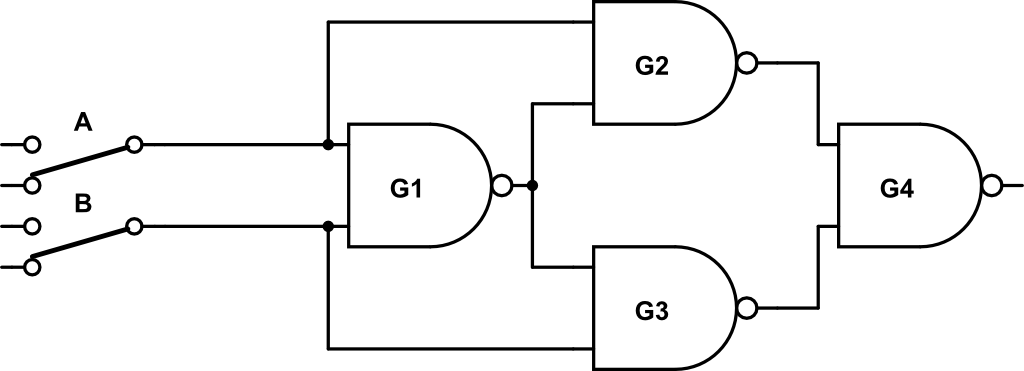
\includegraphics[width=8cm]{../../examples/xor.png}
 \caption{Circuit diagram of an XOR gate implemented using NAND gates}
 \label{fig:example-xor}
\end{figure}

\subsection{4-bit Adder}

\subsubsection{Definition File}
\lstinputlisting[caption=4bitadder.gf2]{../../examples/4bitadder.gf2}

\subsubsection{Circuit Diagram}
\begin{figure}[h]
 \centering
 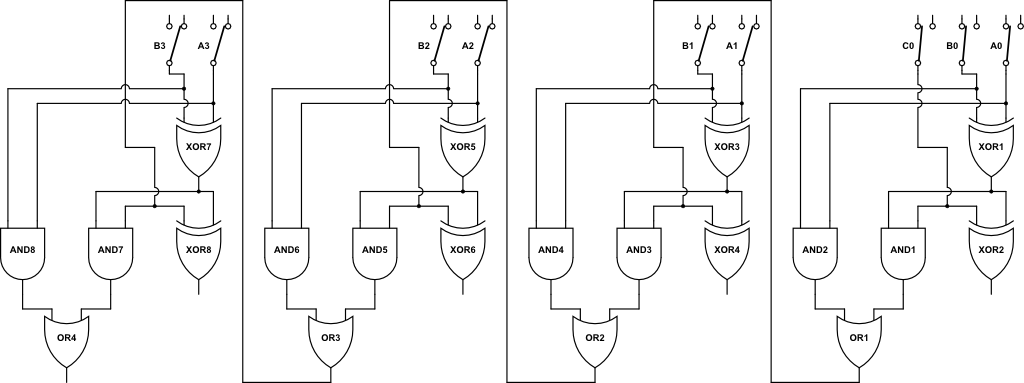
\includegraphics[width=16cm]{../../examples/4-bit-adder.png}
 \caption{Circuit diagram of a 4-bit adder}
 \label{fig:example-adder}
\end{figure}

\subsection{Serial In Parallel Out Shift Register}

\subsubsection{Definition File}
\lstinputlisting[caption=sipo.gf2]{../../examples/sipo.gf2}

\subsubsection{Circuit Diagram}
\begin{figure}[h]
 \centering
 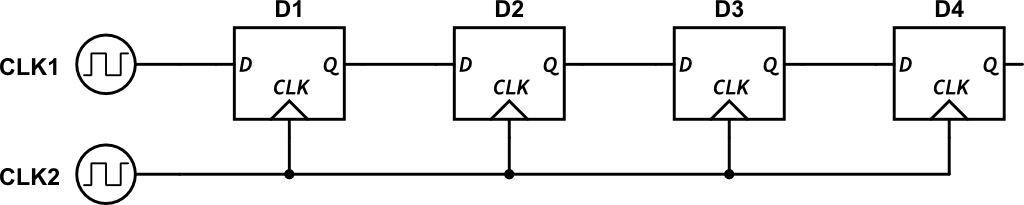
\includegraphics[width=12cm]{../../examples/sipo.png}
 \caption{Circuit diagram of a serial in parallel out shift register}
 \label{fig:example-sipo}
\end{figure}

\textbf{NB} The software used to draw the circuit diagram does not support the same style of D flip-flop used in the definition file, and Fig. \ref{fig:example-sipo} was the closest achievable.

\subsection{Gated D Latch}

\subsubsection{Definition File}
\lstinputlisting[caption=sipo.gf2]{../../examples/gateddlatch.gf2}

\subsubsection{Circuit Diagram}
\begin{figure}[h]
 \centering
 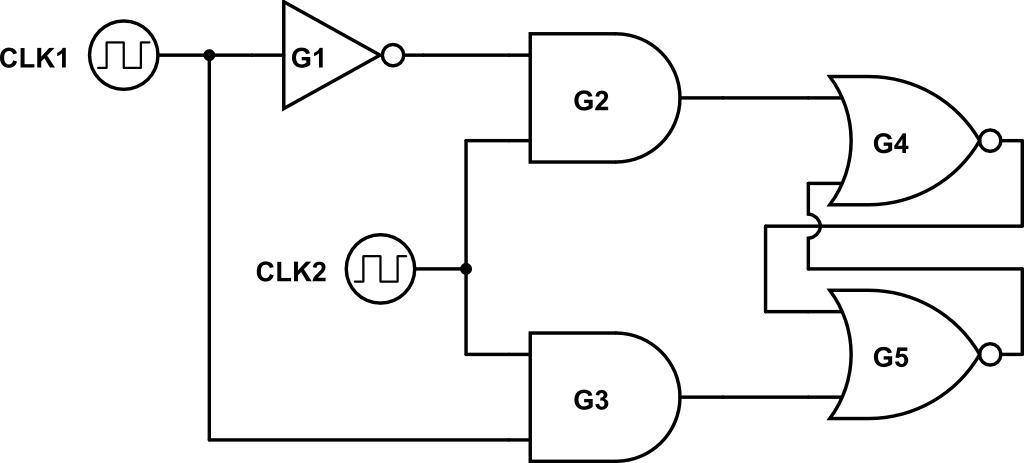
\includegraphics[width=12cm]{../../examples/gated-d-latch.png}
 \caption{Circuit diagram of a Gated D Latch}
 \label{fig:example-dlatch}
\end{figure}

\textbf{NB} The software used to draw the circuit diagram does not support the NAND gates with one input. Therefore the NAND gate G1 was substituted for a NOT gate as can be seen in Fig. \ref{fig:example-dlatch}.

\pagebreak

\section{EBNF}
\lstinputlisting[caption=EBNF]{../../docs/ebnf.txt} %TODO: define EBNF language

\pagebreak

\section{User Guide}

\pagebreak

\section{File Listing}

\end{document}